\chapter{Interactions lumière-matière}
Ce modèle est loin de la réalité mais "correct" en pratique. Il est donc intéressant pour développer une 
certaine intuition du problème.

	\section{Propagation d'onde EM dans un milieu diélectrique}
	\subsection{Approche "particulaire"}
	\begin{wrapfigure}[8]{l}{6cm}
	\vspace{-5mm}
	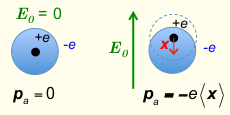
\includegraphics[scale=0.65]{ch2/image1.png}
	\captionof{figure}{ }
	\end{wrapfigure}
	Si la lumière se propage dans un milieu non vide, il y aura des interactions : comment on pourrait décrire 
	ces interactions et d'où elles viennent? Lorsque l'on applique un champ électrique $\vec{E}$ à un système de
	charges, elles ont la possibilité de bouger : le nuage électronique se déforme et il apparaît un moment 
	dipolaire électrique
	\begin{equation}
	\vec{p}_a = -\int e|\psi|^2\vec{r}\ d\vec{r}
	\end{equation}
	où $-e|\psi|^2\ d\vec{r}$ est l'élément de charge à la position $\vec{r}$ donnant lieu à une intégrale 
	non nulle\footnote{Si cette intégrale est nulle lorsque $\vec{E}=\vec{0}$, c'est du au fait que la fonction 
	d'onde est antisymétrique.}. Dans un milieu contenant $N$ atome par unité de volume, la polarisation 
	(macroscopique) est donnée par
	\begin{equation}
	\vec P = N\vec{p_a}
	\end{equation}
	soit la densité atomique multiplié par le moment dipolaire de chaque atome (on suppose que tous les dipôles
	sont orientés dans le même sens).\\
	
	\begin{wrapfigure}[6]{r}{4cm}
	\vspace{-5mm}
	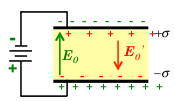
\includegraphics[scale=0.7]{ch2/image2.png}
	\captionof{figure}{ }
	\end{wrapfigure}
	Pour illustrer, penchons-nous sur le cas du condensateur en prenant l'hypothèse d'un milieu linéaire et 
	isotrope (sans quoi la susceptibilité $\chi$ serait un tenseur). Dans ce cas, la polarisation va être
	 proportionnelle à l'amplitude du champ total $E=E_0+E_0'$ où $E_0$ est le champ initial et $E_0'$ le 
	 champ induit.
	 \begin{equation}
	 \left\{\begin{array}{ll}
	 \vec{E_0'} &= -\vec P/\epsilon_0\\
	 \vec E &= \vec E_0-\vec P/\epsilon_0
	 \end{array}\right.\qquad\Rightarrow \vec{P} = \varepsilon_0\chi\vec{E}
	 \end{equation}
	où $\chi$ est la \textbf{susceptibilité électrique}.
	
	Calculons la divergence de ce champ électrique total
	\begin{equation}
	\div \vec{E} = \div(\vec{E_0}-\vec{P}/\epsilon_0)\quad \Leftrightarrow\quad \div(\vec{E}+\vec{P}/\epsilon_0) 
	= \div(\vec{E_0})
	\end{equation}
	Dans le vide $\div(\vec{E_0}) = \rho_{libre}/\epsilon_0$. Pour tenir compte de l'apparition des dipôles, 
	on introduit un \textbf{champ de déplacement} $D$ de sorte à pouvoir écrire une formule de divergence 
	"classique". Par définition
	\begin{equation}
	\vec{D} = \varepsilon_0\vec{E}+ \vec{P} = \varepsilon_0(1+\chi)\vec{E} = \varepsilon\vec{E}
	\end{equation}
	où $\varepsilon_r = \varepsilon/\varepsilon_0 = (1+\chi)$.	On peut alors écrire
	\begin{equation}
	\div\vec{D} = \rho_{libre}
	\end{equation}
	En toute généralité, cette susceptibilité $\chi$ sera complexe : absorption, gain, \dots en découleront.
	
	
	En toute généralité, le champ électrique peut varier dans le temps. On défini alors la \textbf{densité de courant} (densité d'électron * charge * variation de la position de cette charge) :
	$\vec{J}$
	\begin{equation}
	J_{liee} = -Ne\dfrac{d}{dt}\langle x \rangle \quad\Leftrightarrow\quad J_{liee} = N\dfrac{d}{dt}\vec{p_a} =
	\dfrac{d}{dt}\vec{P}
	\end{equation}
	Il y aura toujours un dipôle accompagné d'un moment dipolaire atomique mais cette fois-ci dépendant du temps.\\
	
	
Partons maintenant des équations de Maxwell et des équations constitutives. Considérons 
	un milieu diélectrique ($\rho_{libre}=0$) et non magnétique ($\vec{B}=\mu_0\vec{H}$)
	\begin{equation}
	\left\{\begin{array}{ll}
	\rot\vec{E} &\DS= -\frac{\partial}{\partial t}\vec{B}\\
	\rot\vec{B} &\DS=\mu_0\dfrac{\partial}{\partial t}\vec{D}\\
	\div\vec{D}&=\DS 0\\
	\div\vec{B}&=\DS 0
	\end{array}\right.\qquad\qquad\text{ et }\qquad\qquad\left\{\begin{array}{ll}
	\vec{D} &=\DS \varepsilon\vec{E} = \varepsilon_0\vec{E}+\vec{P}\\
	\vec{B}&=\DS \mu_0\vec{H}
	\end{array}\right.
	\end{equation}
	En calculant le rotationnel du rotationnel du champ électrique\footnote{$\rot\rot = \div\div - \Delta$}, 
	on trouve l'équation d'onde
	\begin{equation}
	\Delta\vec{E}-\frac{1}{c^2}\dfrac{\partial^2}{\partial^2}\vec{E}=\mu_0\dfrac{\partial^2}{\partial t^2}\vec{P}
	\end{equation}
	où $c = 1/\sqrt{\epsilon_0\mu_0}$ est la vitesse de la lumière dans le vide. \\
	
	Trois cas sont particulièrement intéressants
	\begin{enumerate}
	\item	Dans le vide : $\vec{P}=\vec{0}$ et on retrouve la solution harmonique, décrite par des ondes planes
	\begin{equation}
	\vec{E} = \frac{1}{2}(\mathcal{E}\exp(i(\vec{k}.\vec{r}-\omega t))\vec{e} + c.c.)
	\end{equation}
	où $\vec{e}$ est le vecteur de polarisation. Pour que ce soit bien solutions des équations de Maxwell, il 
	faut que $\vec{k}.\vec{e} = 0$ (polarisation transverse) et $|\vec{k}| = \omega/c=2\pi/\lambda_0$.\\
	\item Dans un diélectrique, la polarisation varie dans le temps : effets de réfractions, de perte et de gain
	\item \textbf{Indice de réfraction complexe} $\mathcal{N}$.\\
	Soit la solution harmonique et $\vec{k}=\mathcal{K}.\vec{1_z}$
	Jusqu'ici, nous avons toujours considéré que l'indice de réfraction n'était du qu'à des effets de phase.

	Adoptons des notations en phaseurs
	\begin{equation}
	\vec{E} =\frac{1}{2}(\mathcal{E}\exp(i(\mathcal{K}z-\omega t))\vec{e} + c.c.)= \frac{1}{2}(\hat{\vec{E}}+c.c.),\qquad\qquad\vec{P} = \frac{1}{2}(\hat{\vec{p}}+c.c.)
	\end{equation}
	où nous avons cette fois-ci autorisé $\mathcal{K}$ à être complexe. En faisant de même pour $\hat{\vec{P}}$ 
	(par identification) :
	\begin{equation}
	\hat{\vec{P}} = \varepsilon_0\chi\hat{\vec{E}} = \varepsilon_0(\chi'+i\chi'')\hat{\vec{E}}
	\end{equation}
	Après substitution de ces équations dans l'équation de propagation (la dérivée en $z$ fait apparaître un 
	$\mathcal{K}^2$.
	\begin{equation}
	\mathcal{K}^2 = \dfrac{\omega^2}{c^2}(1+\chi'+i\chi'')
	\end{equation}
	où l'on note $\mathcal{K}=k+i\alpha_E$ où $\alpha_E$ est le coefficient d'atténuation du champ électrique. Si 
	l'on substitue cette nouvelle expression de $\mathcal{K}$ dans l'expression de $\vec{E}$, on fait apparaître 
	une exponentielle négative
	\begin{equation}
	\vec{E}=\mathcal{E}\exp(-\alpha_Ez)\cos(kz-\omega t)
	\end{equation}
	On définit le coefficient d'absorption en énergie $\alpha=2\alpha_E$. Si $\alpha>0$ il s'agit d'un milieu à
	 pertes (à gain, inversement).\\
	 
	Venons-en à ce qui nous intéresse ici : l'\textbf{indice de réfraction complexe} défini
	\begin{equation}
	\mathcal{N} = \eta +i\kappa
	\end{equation}
	tel que $\mathcal{K}=\dfrac{\omega}{c}\mathcal{N}$. Le champ électrique établi ci-dessus devient alors
	\begin{equation}
	\vec{E} =\vec{\mathcal{E}}\exp\left[-\frac{\omega}{c}\kappa z\right]\cos\left(\frac{\omega}{c}\eta z-\omega t\right)
	\end{equation}
	L’absorption vaut alors $\alpha = 2\frac{\omega}{c}\kappa$ et la vitesse de phase $v_\phi = \frac{\omega}
	{c}=\frac{c}{\eta} \to \lambda=\frac{\lambda_0}{\eta}$
	En identifiant la partie réelle et imaginaire :
	\begin{equation}
	\left\{\begin{array}{ll}
	\eta^2-\kappa^2 &= 1+\chi'\\
	\eta\kappa &= \chi''/2
	\end{array}\right.
	\end{equation}
	Souvent on peut entendre que la partie réelle correspond à des effets de phase ($\vec{k}$) alors que la partie 
	imaginaire correspond à des pertes/gain : ce n'est pas exact, les deux sont "mélangés". Cependant, si 
	$\kappa\ll 1$
	\begin{equation}
	\left\{\begin{array}{ll}
	\eta &\approx \sqrt{1+\chi'}\\
	\kappa &\approx \chi''/(2\sqrt{1+\chi'})
	\end{array}\right.
	\end{equation}
	On remarque que $\eta,\kappa$ dépendent de $\omega$. On nomme alors \textbf{relation de dispersion} l'équation $\eta = f(\omega)$.
	\end{enumerate}
	
	\subsection{Modèle de l'oscillateur harmonique}
	Le souci est que nous ne connaissons pas les expression de $\eta, \kappa, \chi'$ et $\chi''$, tous fonction 
	de $\omega$. On va utilisé un modèle qualitativement correct (mais assez loin de la réalité) pour les obtenir 
	dans un milieu diélectrique isotrope (gaz,ions dans un solide,\dots)\\
	
	Considérons \textit{un} électron élastiquement (constante de rappel $k$) lié à un noyau infiniment lourd sur
	lequel on applique $E(t)$. On introduit un terme de relaxation (damping) $m\gamma\dot{x}(t)$ si on veut une
	description assez fidèle, le nuage électronique ne peut osciller infiniment \footnote{Une densité de charge liée
	bougeant agit comme une antenne : émission d'onde EM.}. Il faut donc perdre de l'énergie, ce qui est le rôle de
	ce terme. Nous obtenons alors
	\begin{equation}
	\ddot{x}(t) + \omega_a^2(t)+\gamma\dot{x}(t) = -\frac{eE(t)}{m}
	\end{equation}
	où $\omega_a = \sqrt{k/m}$, $\frac{1}{\gamma}$ est le temps caractéristique de relaxation pour la polarisation 
	$\vec{P}$ et le membre de droite comporte le terme d'oscillation forcée. En utilisant les deux phaseurs
	\begin{equation}
	E(t) = \frac{\mathcal{E}\exp(-i\omega t) + c.c.}{2},\qquad\qquad
	x(t) = \frac{X\exp(-i\omega t) + c.c.}{2}
	\end{equation}
	On trouve
	\begin{equation}
	(\omega_a^2-\omega^2-i\gamma\omega)X\exp(-i\omega t)+c.c. = \frac{e\mathcal{E}}{m}\exp(-i\omega t)+c.c.
	\end{equation}
	Sachant que $\vec{P}=-eN\vec{x}(t)=\frac{\hat{\vec{P}}+c.c.}{2}$ où $\hat{\vec{P}}=\varepsilon_0\chi\hat{
	\vec{E}}$, on trouve
	\begin{equation}
	\chi(\omega) = \dfrac{Ne^2}{\varepsilon_0m}\dfrac{1}{\omega_a^2-\omega^2-i\gamma\omega}
	\end{equation}
	Comme $\chi$ est complexe, il peut y avoir un déphasage entre l'excitation et la position du système 
	masse-ressort
	Les parties réelles et imaginaires valent alors
	\begin{equation}
	\chi'(\omega) = \dfrac{Ne^2}{\varepsilon_0m}\dfrac{\omega_a^2-\omega^2}{(\omega_a^2-\omega^2)^2+\gamma^2
	\omega^2},\qquad\qquad\chi''(\omega) = \dfrac{Ne^2}{\varepsilon_0m}\dfrac{\gamma\omega}{(\omega_a^2-\omega^2)^2+\gamma^2
	\omega^2}
	\end{equation}
	Jusqu'ici, nous travaillons sans approximations mais ces résultats ne sont pas évident à interpréter. Pour 
	se faire, nous allons faire l'hypothèse que l'amortissement est lent. Dès lors, $\vec{E}$ fait un grand 
	nombre d'oscillation avant une atténuation totale du système masse-ressort
	\begin{equation}
	\omega_a^2-\omega^2 = 2\omega_a(\omega_a-\omega)
	\end{equation}
	Avec cette hypothèse, $\chi''$ devient directement proportionnel à $\alpha$ et on le montrera. Il s'agit 
	d'une \textit{lorentzienne}
	\begin{equation}
	\chi''(\omega) = \dfrac{Ne^2}{\varepsilon_0m\gamma\omega_a}\dfrac{1}{1+\frac{(\omega_a-\omega)^2}{(\gamma
	/2)^2}} > 0
	\end{equation}
	
	\begin{wrapfigure}[6]{l}{6.5cm}
	\vspace{-5mm}
	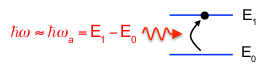
\includegraphics[scale=0.7]{ch2/image3.png}
	\captionof{figure}{ }
	\end{wrapfigure}
	Cette fonction est positive $\forall\omega$, ce qui implique que $\alpha$ sera toujours positif ce qui 
	correspond à de l'absorption : passage d'un niveau fondamental vers un état excité.\\
	Pour $\chi'(\omega)$, on trouve
	\begin{equation}
	\chi'(\omega) = \dfrac{Ne^2}{\varepsilon_0m\gamma\omega_a}\dfrac{(\omega_a-\omega)/(\gamma/2)}
	{1+\frac{(\omega_a-\omega)^2}{(\gamma	/2)^2}}
	\end{equation}
	Ceci met en évidence une variation de l'indice de réfraction : c'est une relation de dispersion. 
	
	\newpage
	Traçons ces deux courbes. Ci-dessous, en rouge, nous avons une absorptions. En vert, une variation de
	l'indice de réfraction : nous verrons que s'il y a un effet d’absorption, il y a forcément un effet 
	de réfraction $\eta$ alors que $\kappa \propto \chi''(\omega)$
	\begin{center}
	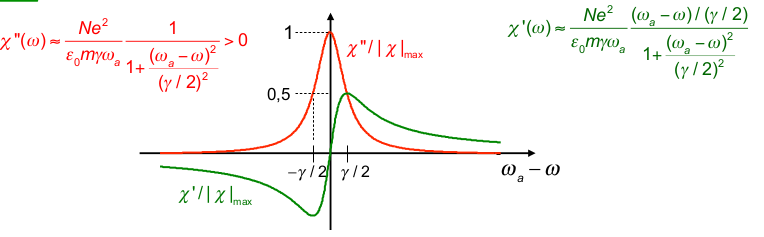
\includegraphics[scale=0.5]{ch2/image4.png}
	\captionof{figure}{ }
	\end{center}	
	Si l'on excite le système en balayant sur les fréquences, nous observerons des pics d'absorption 
	($\kappa$) et une modification de $\eta$. Le verre se situe entre deux pics : il est transparent 
	car il n'y a pas d’absorption par contre on observe tout de même une variation de l'indice de 
	réfraction permettant de distinguer les différentes couleurs.
	\begin{center}
	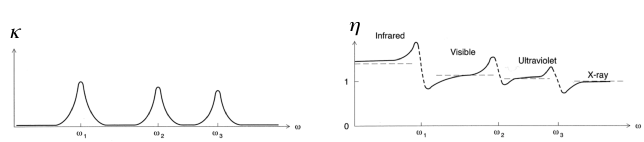
\includegraphics[scale=0.7]{ch2/image5.png}
	\captionof{figure}{ }
	\end{center}	
	
	\newpage
	\section{Particule de lumière}
	\subsection{Équations de Maxwell : onde électromagnétique}
	Jusqu'ici nous avons utilisé une approche électromagnétique : passons cette fois-ci à une approche
	corpusculaire. Intéressons-nous à l'énergie (ce qui est quantifié). On s'intéresse à l'intensité ($W
	/m^2$) qui est liée au vecteur de Poyting $\vec{\mathcal{S}}=\vec{E}\times\vec{H}$ et on en prend la
	moyenne\footnote{Un flux d'énergie oscillant n'a pas de sens.} 
	\begin{equation}
	I = \langle|\vec{\mathcal{S}}|\rangle = \langle|\vec{E}\times\vec{H}\rangle = \frac{1}{2}\varepsilon_0
	\eta\mathcal{E}^2
\end{equation}		
	La solution harmonique des équations de Maxwell étant
	\begin{equation}
	\vec{E} = \mathcal{E}\cos(kz-\omega t)\vec{e}
	\end{equation}
	Nous remarquons qu'il n'y a aucune condition sur l'amplitude $\mathcal{E}$ qui peut varier de façon 
	continue : de même pour l'intensité. Toutes les énergies seraient alors possibles ce qui est faux 
	expérimentalement (effet photoélectrique notamment). 
	
	\subsection{Lumière : un ensemble de photons}
	Planck par l'étude du corps noir et Einstein avec l'effet photoélectrique ont proposés une quantification
	du champ électromagnétique : les quanta de lumières ont une énergie $\Delta E = \hbar\omega$.
	
	\subsection{Description simplifiée de la quantification des champs EM}
	\begin{wrapfigure}[10]{l}{7.5cm}
	\vspace{-5mm}
	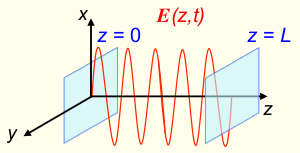
\includegraphics[scale=0.7]{ch2/image6.png}
	\captionof{figure}{ }
	\end{wrapfigure}
	Supposons une cavité vide (pas de radiation, charge, milieu diélectrique), unidimensionnelle selon $z$ 
	formée de murs parfaitement conducteurs (un miroir parfait, rien ne sort de la cavité) en $z=0,L$ où passe
	 un champ $\vec{E}$ polarisé selon $x$. Nous allons toujours appliquer les équations de Maxwell, mais avec 
	 ces conditions de cavité
	\begin{equation}
	\dfrac{\partial^2}{\partial z^2}E_x(z,t) -\frac{1}{c^2}\dfrac{\partial^2}{\partial t^2}E_x(z,t)=0
	\end{equation}
	avec comme CL $E_x=0$ en $z=0,L$. La solution n'est rien d'autre que l'harmonique
	\begin{equation}
	E_x(z,t) = f_0\sin(kz)q(t),\qquad k=\frac{m\pi}{L};\quad m=1,2,\dots
	\end{equation}
	où $E_x$ dépend de $z$ et $t$, $f_0$ est l'amplitude multipliée par la variation spatiale et par une 
	fonction non définie. C'est exactement ce que nous avions obtenu (et heureusement, nous décrivons la 
	même chose). On en tire facilement le champ magnétique
	\begin{equation}
	B_y(z,t) = \frac{\mu_0\varepsilon_0}{k}f_0\cos(kz)\dot{q}
	\end{equation}
	où $\dot{q} =\frac{dq}{dt}$. Ces deux équations, pour $m$ fixé, forment un \textbf{mode de cavité} pour 
	le champ électromagnétique de fréquence angulaire $\omega = m\pi c/L$.\\
	
	Intéressons-nous à l'énergie totale d'un mode : il s'agit de la densité d'énergie du champ magnétique 
	et du champ électrique. 
	\begin{equation}
	H = \int\left[\frac{1}{2}\varepsilon_0E_x^2+\frac{1}{2\mu_0}B_y^2\right]\ dV
	\end{equation}
	Sachant que $V$ est le volume effectif de la cavité, on trouve
	\begin{equation}
	H = \frac{1}{4}f_0^2\varepsilon_0V\left[\dfrac{\varepsilon_0\mu_0}{k^2}\dot{q}^2\right]
	\end{equation}
	Pour simplifier, on considère la constante de normalisation $\DS f_0=\left(\dfrac{2\omega^2}{
	\varepsilon_0V}\right)^2$ :
	\begin{equation}
	H = \frac{1}{2}(p^2+\omega^2q^2)
	\end{equation}
	Ce qui n'est rien d'autre que l'Hamiltonien de l'oscillateur harmonique où $q$ est la position de la 
	masse et où la force de rappel est $F=-\omega^2 q$ (et $p=\dot{q}$). Par analogie, un mode de champ 
	électromagnétique est équivalent à un oscillateur harmonique qui aurait une masse unitaire et où les 
	champs $\vec{E}$ et $\vec{B}$ jouent le même rôle que la position et le moment. L'idée venant 
	naturellement est alors d'essayer de quantifier cette O.H. en utilisant le principe de correspondance 
	$p\to\hat{p}, q\to\hat{q}$ tel que $\hat{p}=-i\hbar \nabla$. \\
	
	Passons donc en mécanique quantique sans se soucier que $H$ est l'énergie d'un cas classique. L'équation 
	de Schrödinger indépendante du temps s'écrit
	\begin{equation}
	\left(\dfrac{\hbar^2}{2}\dfrac{d}{dq^2}+\dfrac{\omega^2}{2}q^2\right)\phi(q) = E\phi(q)
	\end{equation}
	On trouve comme énergie quantifiée
	\begin{equation}
	E_n = \left(n_p+\dfrac{1}{2}\right)\hbar\omega
	\end{equation}
	où on va interpréter $n_p$ comme le nombre de photons contenus dans la cavité considérée. On nomme 
	$E_0$ les \textit{fluctuations du vide} qui peuvent être utile mais pas ici : comme nous allons 
	sommer une infinité de mode, on obtiendrait une énergie infinie. On n'en tiendra donc pas compte.\\
	
	Nous n'avions pas définit $q(t)$ : il s'agit d'une fonction évoluant au cours du temps : celle-ci donnera 
	l'amplitude du champ. L'énergie contenue dans le champ est ainsi proportionnelle au carré de l'amplitude 
	de ce champ ce qui n'est rien d'autre que le cas classique où chaque oscillateur est défini par $\omega, 
	\vec{k}$.
	\begin{equation}
	\langle q\rangle = \bra{\phi}q\ket{\phi} = 0,\qquad\qquad\qquad \langle q^2\rangle\propto E_n
	\end{equation}
	
	\subsection{Flux de photon $\mathcal{J}$ et densité $n_p$}
		\begin{wrapfigure}[6]{l}{7.5cm}
	\vspace{-5mm}
	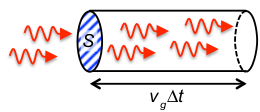
\includegraphics[scale=0.7]{ch2/image7.png}
	\captionof{figure}{ }
	\end{wrapfigure}
	Nous allons suivre la démarche de Planck, à savoir tenter de quantifier le corps noir. Supposons que les 
	photons soient monochromatiques et qu'ils se déplacent à la vitesse de groupe
	\begin{equation}
	v_g = \frac{c}{n_g} = \left(\dfrac{\partial k}{\partial\omega}\right)^{-1}
	\end{equation}
	Il est dès lors utile de s'intéresser au flux du photon car l'intensité peut facilement s'en déduire : 
	l'intensité est donnée par le produit de l'énergie d'un photon par le flux photonique. La valeur moyenne
	du vecteur de Poynting donne l'intensité\footnote{Pq $\mathcal{J}\hbar\omega$ ?}
	\begin{equation}
	\langle |\vec{S}|\rangle = \mathcal{J}\hbar\omega = \frac{1}{2}\varepsilon_0c\eta\mathcal{E}^2 = I\qquad
	\Leftrightarrow\qquad \mathcal{J} = \dfrac{\eta\varepsilon_0c}{2\hbar\omega}\mathcal{E}^2
	\end{equation}
	où $\mathcal{J}$ est le \textbf{flux de photon} [$m^{-2}.s^{-1}$]. On a donc un lien direct entre le flux 
	de photon et le module carré de l'amplitude du champ. A l'aide du schéma ci-dessus, nous pouvons montrer 
	que la \textbf{densité de photon} [$m^{-3}$]vaut 
	\begin{equation}
	\mathcal{J}S\Delta t = n_pSv_G\Delta t\qquad\Leftrightarrow\qquad n_p = \dfrac{\mathcal{J}}{v_g}=
	\dfrac{\eta n_g\varepsilon_0}{2\hbar\omega}\mathcal{E}^2
	\end{equation}
	ce qui n'est \textbf{pas} $n_p$ (nombre de photons).
	
	\section{Cavité radiative}
	Le but est d'obtenir la densité d'énergie par unité de fréquence d'un corps noir. Ce que l'on va faire pour 
	y parvenir, c'est faire un tout petit trou en supposant que l'équilibre thermique n'est pas perturbé, et 
	observer ce qui sort. Planck a ainsi trouvé que la probabilité de trouver un mode à une certaine énergie 
	donnée est donné par la loi de Boltzmann. \\
	La probabilité $p_{np}$ qu'un mode (oscillateur) soit dans l'état $n_p$ est donné par
	\begin{equation}
	p_{n_p} = \dfrac{\exp(-E_{n_p}/k_BT)}{\sum_{n_p=0}^\infty \exp(-E_{n_p}/k_BT)}
	\end{equation}
	où la division par la série permet la normalisation et où $E_{n_p} = (n_p+1/2)\hbar\omega$. Après 
	substitution
	\begin{equation}
	p_{n_p} = \dfrac{\exp(-n_p\hbar\omega/k_BT)}{\sum_{n_p=0}^\infty \exp(-n_p\hbar\omega/k_BT)}
	\end{equation}
	Le nombre moyen de photon est donné par l'espérance mathématique. En adoptant la notation
	\begin{equation}
	\langle n_p\rangle = \sum_{n_p=0}^\infty n_pp_{n_p},\qquad x=\dfrac{\hbar\omega}{k_BT}
	\end{equation}
	On trouve
	\begin{equation}
	\langle n_p\rangle = \dfrac{\sum_{n_p=0}^\infty n_p\exp(-n_p\hbar\omega/k_BT)}{\sum_{n_p=0}^\infty \exp(-n_p\hbar\omega/k_BT)}
	\end{equation}
	Le résultat (numérique et graphique) après résolution des séries est donné ci-dessous.\newpage
	\begin{center}
	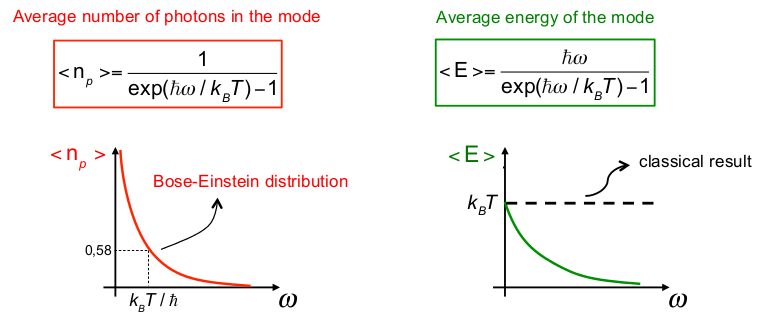
\includegraphics[scale=0.55]{ch2/image8.png}
	\captionof{figure}{ }
	\end{center}
	Le nombre moyen de photons dans un mode est donné par la distribution de Bose-Einstein : sa multiplication 
	par $\hbar\omega$ donne l'énergie moyenne du mode. Il s'agit d'une fonction décroissante tendant vers 
	$k_BT$ lorsque $\omega\to0$.\\
	
	Si l'on effectue le calcul, à température ambiante, il y a à peu près $e^{-100}$ photons visible : ceci 
	est cohérent avec le fait que la lumière ne rayonne pas. Dans un cadre classique, Rayleigh-Jeans avaient 
	obtenu (variation continue d'énergie)
	\begin{equation}
	\langle E\rangle = \dfrac{\int_0^\infty Ee^{-E/k_BT}\ dE}{\int_0^\infty e^{-E/k_BT}\ dE} = k_BT
	\end{equation}
	Ceci est vrai à faible fréquences, mais totalement faux à hautes fréquences.
	
	\subsection{Spectre de la cavité radiative}
	Connaître l'énergie dans un mode n'est que peu intéressant si l'on ne sait pas combien il y a de mode
	par unité de fréquence. On va émettre l'hypothèse que le spectre de la radiation du corps noir est 
	proportionnel à la \textbf{densité spectrale d'énergie} $u(\omega)$ dans la cavité. On va utiliser
	\begin{equation}
	u(\omega)\ d\omega
	\end{equation}
	Il s'agit de la multiplication entre l'énergie moyenne dans un mode par la densité spectrale\footnote{"Combien 
	j'ai de mode par unité de volume par fréquence $\omega$"} en 	énergie, soit le nombre de mode par unité de
	volume dans un intervalle $[\omega,\omega+d\omega]$. Dès lors
	\begin{equation}
	u(\omega)d\omega = \langle E\rangle \rho(\omega)d\omega
	\end{equation}
	\begin{wrapfigure}[6]{r}{4.5cm}
	\vspace{-5mm}
	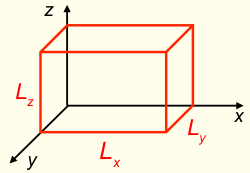
\includegraphics[scale=0.5]{ch2/image9.png}
	\captionof{figure}{ }
	\end{wrapfigure}
	où $\rho(\omega)$ est la densité spectrales des mode dans le champ EM. Intéressons-nous aux nombres de 
	mode par unité de fréquence par unité de volume $\rho(\omega)$ d'une cavité rectangulaire de volume 
	$V=L_1L_2L_3$ (on va montrer que c'est indépendant de la géométrie) composée de murs parfaitement 
	conducteurs et à l'équilibre thermique à la température $T$.
	\newpage
	
	Le slide 19 donne la résolution (par séparation de variable) de ce problèmes aux limites. Si l'on fixe 
	$l,m$ et $n$ le vecteur d'onde est fixé : il y aura deux solutions possibles correspondant à deux 
	polarisations orthogonales. 
	\begin{equation}
	k_x = \frac{l\pi}{L_x},\qquad k_y = \frac{m\pi}{L_y}, \qquad k_z = \frac{n\pi}{L_z}
	\end{equation}
	où $l,m,n=0,1,2,\dots$. Nous pouvons maintenant calculer le nombre de mode présent dans l'intervalle 
	de fréquences $[\omega,\omega+d\omega]$ : ce calcul est plus simple dans l'espace réciproque car une 
	cellule de cette espace à les dimensions $\pi/L_x, \pi/L_y, \pi/L_z$. En notant ce nombre de mode $N_k$, 
	on trouve
	\begin{equation}
	N_k = 2\dfrac{1}{8}\dfrac{4\pi k^2\ dk}{8\frac{\pi}{L_x}\frac{\pi}{L_y}\frac{\pi}{L_z}} = \dfrac{k^2\ dk}
	{\pi^2}V
	\end{equation}
	où nous avons deux états de polarisation, le facteur $1/8$ correspond au huitième de sphère et où l'on a 
	divisé le volume de la calotte sphérique par le volume d'une cellule élémentaire. Sachant que $k^2 =
	\omega^2/c^2 \rightarrow k\ dk = \omega d\omega/c^2$
	\begin{equation}
	\frac{N_\omega}{V} = \rho(\omega)d\omega = \frac{\omega}{c}\frac{\omega d\omega}{\pi^2 c^2}
	\end{equation}
	où nous avons divisé par le volume, voulant une densité. Après intégration, on trouve la densité spectrale 
	de mode
	\begin{equation}
	\rho(\omega) = \dfrac{\omega^2}{\pi^2c^3}
	\end{equation}
	En multipliant par l'énergie moyenne (espérance mathématique), on trouve la \textbf{loi de radiation de 
	Planck}
	\begin{equation}
	u(\omega) = \dfrac{\hbar\omega^3}{\pi^2c^3}\dfrac{1}{e^{\hbar\omega/k_BT}-1}
	\end{equation}
	
	\begin{wrapfigure}[10]{r}{6.5cm}
	\vspace{-5mm}
	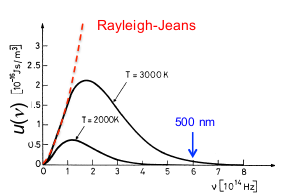
\includegraphics[scale=0.65]{ch2/image10.png}
	\captionof{figure}{ }
	\end{wrapfigure}
	
	Cette expression est en excellent accord avec l'expérience, impliquant une quantification du champ EM. 
	Cette loi n'est strictement valable que pour une cavité fermée en équilibre thermique. Cependant, elle 
	décrit bien les radiations de sources thermiques non nécessairement à l'équilibre thermique, comme le 
	soleil. Si la cavité n'est pas vide (diélectrique) il suffit de remplacer $c$ par $c/\eta$. La 
	généralisation est immédiate
	\begin{equation}
	u(\omega) = \dfrac{\hbar\omega^3\eta^3}{\pi^2c^3}\dfrac{1}{e^{\hbar\omega/k_BT}-1}
	\end{equation}
	Il est possible d'obtenir une telle courbe pour le spectre du soleil. Le seul paramètre libre étant la 
	température, il a été possible de mesurer la température du soleil sans devoir y tremper son doigt. Si 
	l'on regarde la courbe de radiation du corps noir à $T=2.726\ K$ on se rend compte que la courbe 
	ne peut pas plus coller les prédictions expérimentales.
	
	
	
	\newpage
	\section{Interactions dans un milieu à deux niveaux atomiques}
	
	
	
	
	
	
	
	
	
	
	
	
	
	